% !TeX spellcheck = cs_CZ
%{\tikzset{external/prefix={tikz/CES/}}
% \tikzset{external/figure name/.add={ch09_}{}}
%---------------------------------------------------------------------------------------------------
% file STM32F100VL_Kit.tex
%---------------------------------------------------------------------------------------------------
%==============================Kapitola: STM32 VL Discovery=========================================
\setchaptertoc
\chapter{Vývojový kit STM32F4 Discovery}

  Vývojové desky pro STM mikrokontroléry založené na ARM CortexM4 jádře, poskytují základy pro 
  budování široké škály vestavěných (\wikiEmbedded) systémů od jednoduchých bateriových klíčů až po 
  složité systémy pracující v reálném čase (autopilot vrtulníku, atd.). Vývojové kity STM32F4 
  Discovery, jsou díky své ceně také velice populární mezi amatérskými konstruktéry.
  
  Součástí kitu jsou i programové vybavení v podobě knihoven pro ovládání všech periferií 
  mikrokontroléru a také různých senzorů (akcelerometr, atd.), které jsou již součástí kitu.  
  Tato kapitola je navazuje 
  s programovacími zkušenostmi "C", ale žádné předchozí zkušenosti s vloženým programem
  systémy.
  
  \section{Charaketristika vývojové desky}
    Programování ARM procesorů se nejdříve vyzkoušíme na vývojovém kitu \textbf{STM32 Value Line 
    Discovery} (obr.\ref{MIT:fig_stm32vlkit}) firmy ST Microelectronics. Tento kit je osazen 
    32-bitovým procesorem \texttt{STM32F100RB} patřící do rodiny \texttt{Cortex-M3}, jenž je 
    založena na architektuře jádra \texttt{ARMv7} (obr. \ref{MIT:fig_stm32f100arch}). 
  
    \begin{figure}[ht!] %\ref{MIT:fig_stm32vlkit}
      \centering
      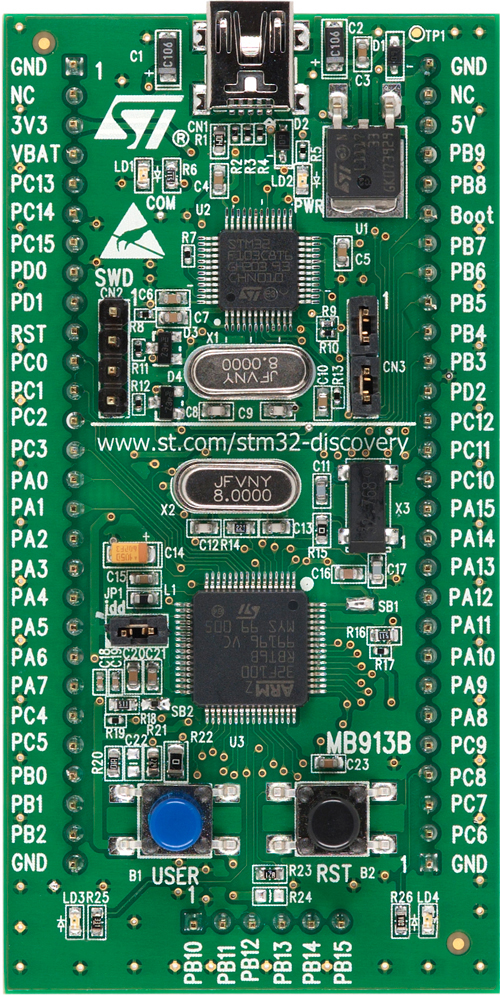
\includegraphics[width=0.7\linewidth]{board_stm32vl_discovery.jpg}
      \caption{STM32VL Discovery kit}
      \label{MIT:fig_stm32vlkit}
    \end{figure}
    
    \subsection{Doporučená literatura}:
    \begin{itemize}
      \item \href{http://librarian/stable.php?id=143}{Discovering the STM32 Microcontroller}: 
            kniha je praktickou příručku pro pochopení programování rodiny mikrokontrolerů 
            \texttt{STM32} \texttt{F1}. Tato příručka byla napsána, pro podporu mladší-rovný kurs 
            počítačové vědy v 
      Indianské univerzitě. 
    \end{itemize}
  
    Kit se skládá ze dvou částí. Horní část na obr. \ref{MIT:fig_stm32_desc} se nazývá 
    \texttt{ST-Link} (obsahuje ARM čip STM32F103C8T6) a je určena k programování a ladění vlastního 
    \texttt{Value Line} mikroprocesoru typu \textbf{STM32F100RBT6} (dále jen \texttt{MCU VL}) 
    umístěného na druhé spodní polovině.
  
    Kit obsahuje 4 LED, z toho 2 LED slouží pro ST-Link část a dvě tlačítka, z toho jedno je určeno 
    pro RESET \texttt{MCU VL}:
    \begin{itemize}[noitemsep]
      \item {\color{red} \textbf{LD1}}: na DPS značena jako \texttt{COM}, signalizuje komunikaci 
            mezi \texttt{PC} a \texttt{ST-Link} rozhraním;
      \item {\color{red} \textbf{LD2}}: značena jako \texttt{PWR} indikuje napájení kitu.
      \item {\color{blue} \textbf{LD3}}: značena jako \texttt{PC9} je připojena k pinu \texttt{PC9 
             MCU VL};
      \item {\color{green} \textbf{LD4}}: značena jako \texttt{PC8} je připojena k pinu   
            \texttt{PC8 MCU VL};
      \item \textbf{B1}: značeno jako \texttt{USER} je připojeno k pinu \texttt{PA0 MCU VL} a může 
            být použito ve funkci \texttt{WAKE-UP}.
      \item \textbf{B2}: značeno jako \texttt{RST} a je určeno pro reset \texttt{MCU VL}.
    \end{itemize}
    
    Napájení \texttt{VL MCU U3} je vedeno přes propojku \texttt{JP1} (viz obr. 
    \ref{MIT:fig_stm32_desc}). Výhodou této propojky je, že můžeme změřit spotřebu VL MCU, když 
    místo 
    propojky zapojíme ampérmetr.
    \begin{figure}[ht!] %\ref{MIT:fig_stm32_desc}
      \centering
      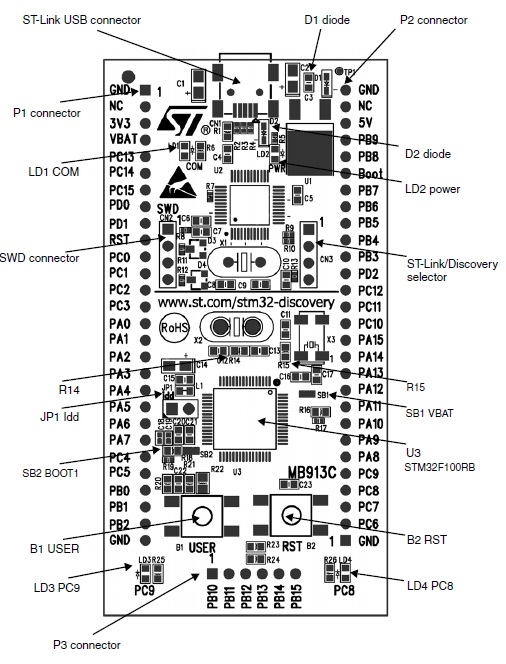
\includegraphics[width=0.9\linewidth]{board_stm32vl_desc.jpg}
      \caption{STM32VL Discovery kit - součásti kitu}
      \label{MIT:fig_stm32_desc}
    \end{figure}
    
    \begin{itemize}[noitemsep]
      \item \href{http://librarian/stable.php?id=142}{Obvodové schéma}
    \end{itemize}
    
    \subsection{Blikáme s LED}
      Naším prvním úkolem je rozblikat LED LD3 připojenou na pin PC9. Je to sice jednoduchý úkol, 
      ale 
      nejsnáze na něm pochopíme, jak se pracuje GPIO jednotkou. Výchozím zdrojem informací pro nás 
      bude obsáhlá referenční příručka RM0041, ve které jsou popsány registry všech periferií 
      mikroprocesorů typu STM32F100.

%} % tikzset
%---------------------------------------------------------------------------------------------------